\documentclass{beamer}

\usepackage[T1]{fontenc}
\usepackage[utf8]{inputenc}
\usepackage[english]{babel}
\usepackage{lmodern}
\usepackage{graphicx}
\usepackage{wrapfig}
\usepackage{animate}

% Use Unipd as theme, with options:
% - pageofpages: define the separation symbol of the footer page of pages (e.g.: of, di, /, default: of)
% - logo: position another logo near the Unipd logo in the title page (e.g. department logo), passing the second logo path as option
% Use the environment lastframe to add the endframe text
\usetheme[pageofpages = of]{Unipd}

\title[]{Hardware/Software Design and Implementation of an Open Robotic Chain Using Custom Servo-Motor Modules}
\subtitle{}
\author[Filippo Gottardo]{ % Argomento opzionale per il piè di pagina
    \texorpdfstring{ % Inizio comando magico
        % --- VERSIONE GRAFICA (per la slide) ---
        \parbox{\linewidth}{
            % Colonna Sinistra: Relatori
            \begin{minipage}[t]{0.5\linewidth}
                \raggedright
                \footnotesize
                \textbf{Supervisor:}\\
                Prof. Angelo Cenedese\\[0.5em]
                \textbf{Co-supervisor:}\\
                Ing. Riccardo Antonello
            \end{minipage}%
            \hfill
            % Colonna Destra: Candidato
            \begin{minipage}[t]{0.45\linewidth}
                \raggedleft
                \textbf{Candidate:}\\
                Filippo Gottardo
            \end{minipage}
        }
    }{Filippo Gottardo} % --- VERSIONE TESTO (per i metadati PDF, invisibile) ---
}

\date{December 4, 2025}


\begin{document}

% Make the title page
\frame{\titlepage}

% Insert the general toc
\begin{frame}{Table of Contents}
    \tableofcontents
\end{frame}

\section{Thesis Objective}

    \begin{frame}{Thesis Objectives}
        \begin{columns}[c]
            \begin{column}{0.5\textwidth}
                \centering
                Design and implement a 3-DOF robotic limb for a bio-inspired walking hexapod.

                \vspace{10pt}
                \textbf{Tracking accuracy}

                \vspace{10pt}
                \textbf{Accessible budget}

                \vspace{10pt}
                \textbf{Modular design}
            \end{column}

            \begin{column}{0.50\textwidth}
                \centering
                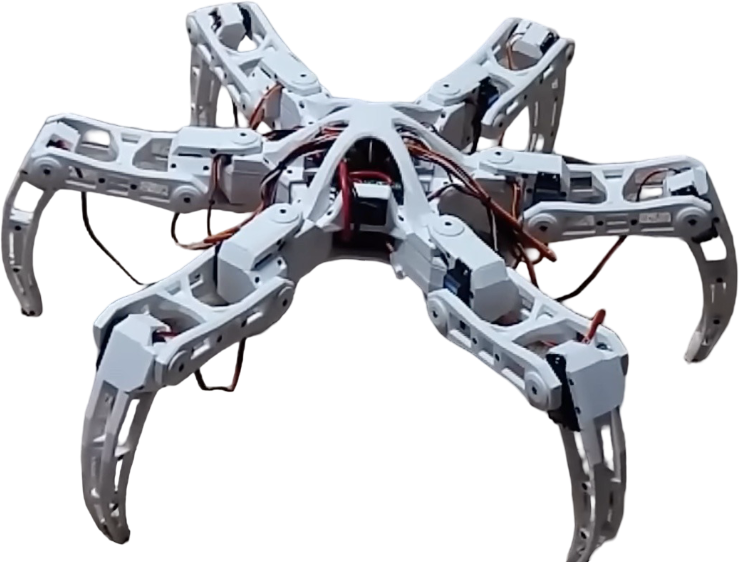
\includegraphics[width=\textwidth]{hexapod.png}
            \end{column}
        \end{columns}
    \end{frame}


\section{Actuator Module}

    \begin{frame}{Commercial Actuator}
        \begin{columns}[c]
            \begin{column}{0.5\textwidth}
                \centering
                \textbf{MG996R servo motor}
                \vspace{10pt}
                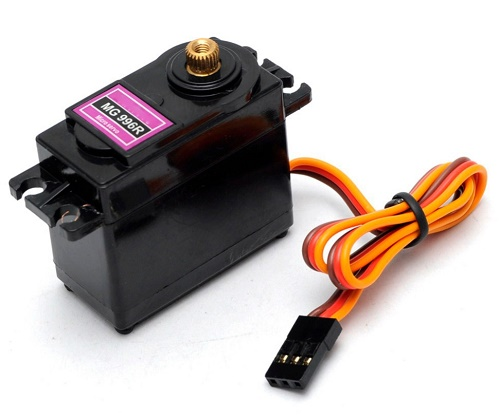
\includegraphics[width=0.6\textwidth]{motor.jpg}

                Non-linear
                \vspace{10pt}

                Backlash/Hysteresis
                \vspace{10pt}

                $\theta_A(T_{on})\ne\theta_B(T_{on})$
                \vspace{10pt}

                No access to $\theta$

            \end{column}

            \begin{column}{0.50\textwidth}
                \centering
                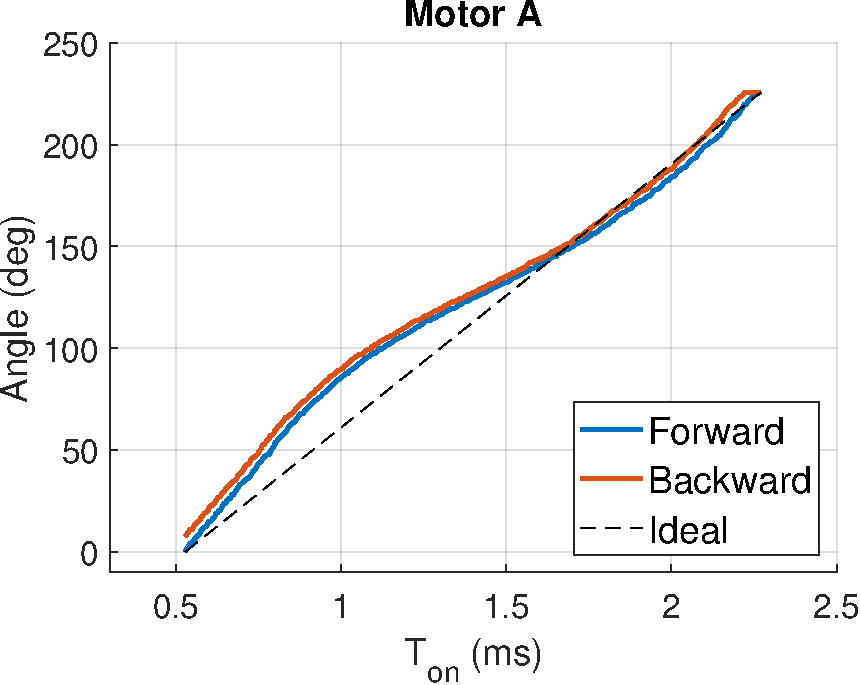
\includegraphics[width=0.8\textwidth]{motor_char_A.pdf}
                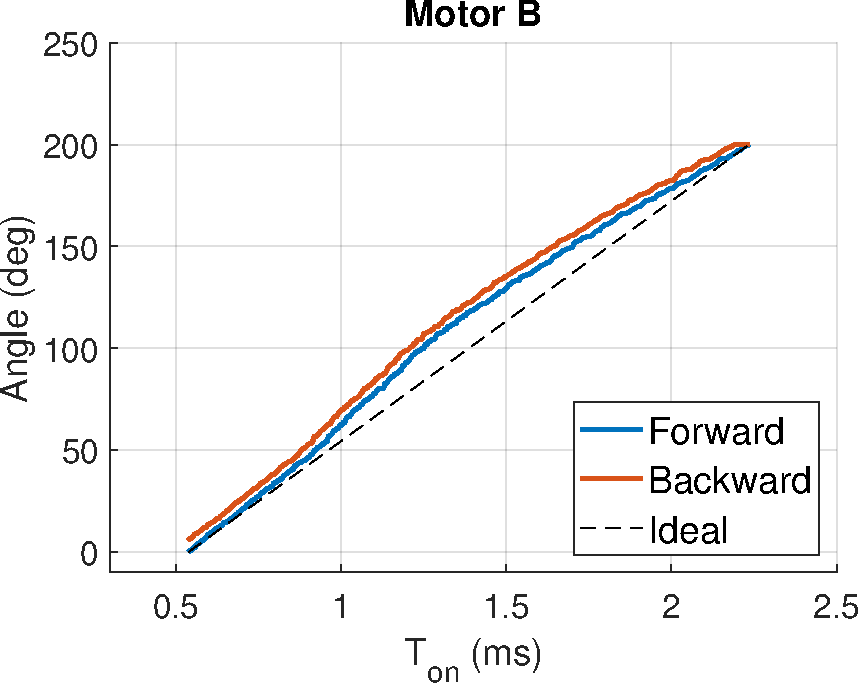
\includegraphics[width=0.8\textwidth]{motor_char_B.pdf}
            \end{column}
        \end{columns}
    \end{frame}

    \begin{frame}{Custom Redesign}
        \centering
        HW/SW Redesign
        \begin{columns}[b]
            \begin{column}{0.50\textwidth}
                \centering
                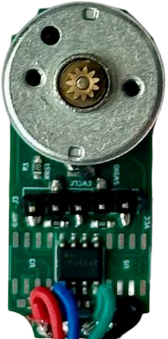
\includegraphics[width=0.48\linewidth]{bottom_motor.png}% <--- Importante questo %
                \hfill
                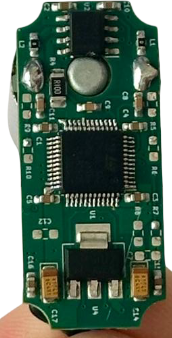
\includegraphics[width=0.48\linewidth]{front_motor.png}

                Potentiometer $\Rightarrow$ Magnetic Encoder
                \vspace{10pt}

                STM32 Microcontroller
            \end{column}

            \begin{column}{0.5\textwidth}
                \centering
                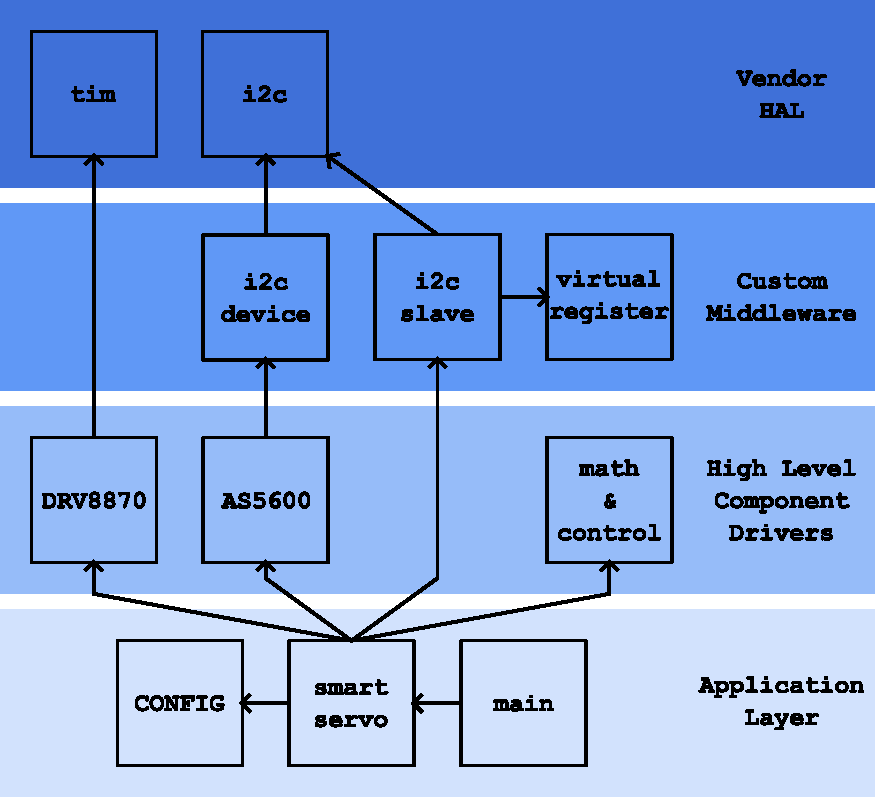
\includegraphics[width=\textwidth]{software_architecture.pdf}

                Switching PID
                \vspace{10pt}

                PWM signal $\Rightarrow I^2C$ Bus Protocol
            \end{column}
        \end{columns}
    \end{frame}

    \begin{frame}{Switching PID}
        \begin{columns}[c]
            \footnotesize
            \begin{column}{0.5\textwidth}
                \centering
                Generalized Position Error: $\sigma = K_I(\theta_d - \theta)$\\

                \vspace{20pt}
                Controller State: $\phi = K_P(\theta_d - \theta) + \frac{K_I \sigma}{s}$\\

                \vspace{20pt}
                Controller Output: $u = \phi - K_Dv$\\

                \vspace{20pt}
                $K_P, K_I > 0, K_PK_D > K_I$\\

                \vspace{20pt}
                $[K_P, K_I, K_D]^T = [10, 0.9, 0.1]^T$
            \end{column}

            \begin{column}{0.5\textwidth}
                \centering
                During stick phase, $v = 0, \sigma(t) = \sigma, -F_- \le \phi \le +F_+$.\\

                \vspace{20pt}
                Integral action $\phi$ accumulates energy to overcome static friction.\\

                \vspace{20pt}
                Once motion begins, if the position errors surpasses the set-point, $\phi \gets -\phi$.\\
            \end{column}
        \end{columns}

        \vspace{20pt}

        \tiny
        "To stick or to slip: A reset PID control perspective on positioning systems with friction"\\
        A. Bisoffi, R. Beerens, W. Heemels, H. Nijmeijer, N. van de Wouw, and L. Zaccarian\vspace{10pt}

        "Switching pid strategy for positioning systems with non-symmetric friction and noisy velocity measurements"\\
        R. Lorigiola, T. Borzone, M. Bruschetta, and A. Cenedese
    \end{frame}

    \begin{frame}{Redesign Results}
        \begin{columns}[c]
            \begin{column}{0.38\textwidth}
                \centering
                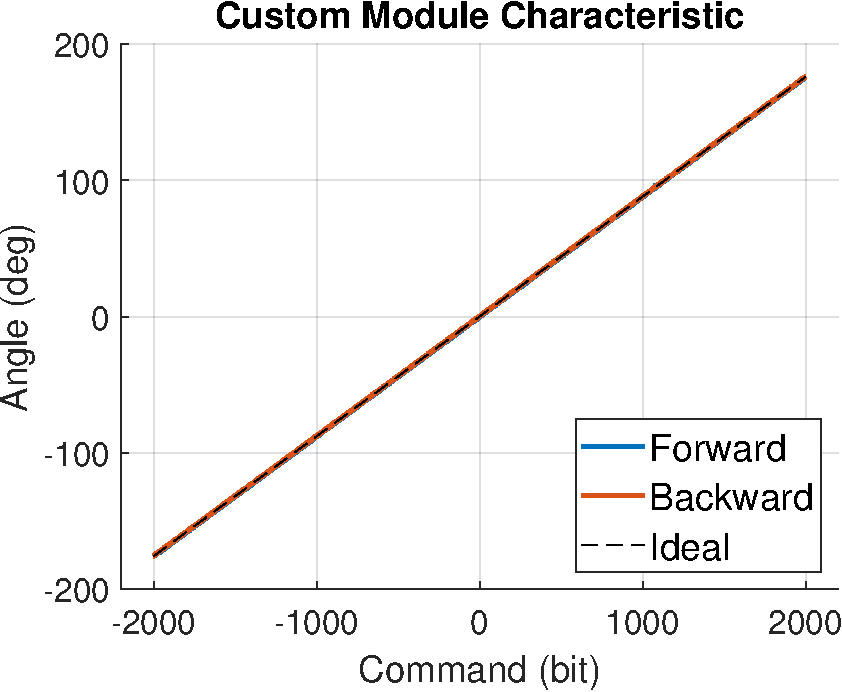
\includegraphics[width=\textwidth]{custom_linearity.pdf}
                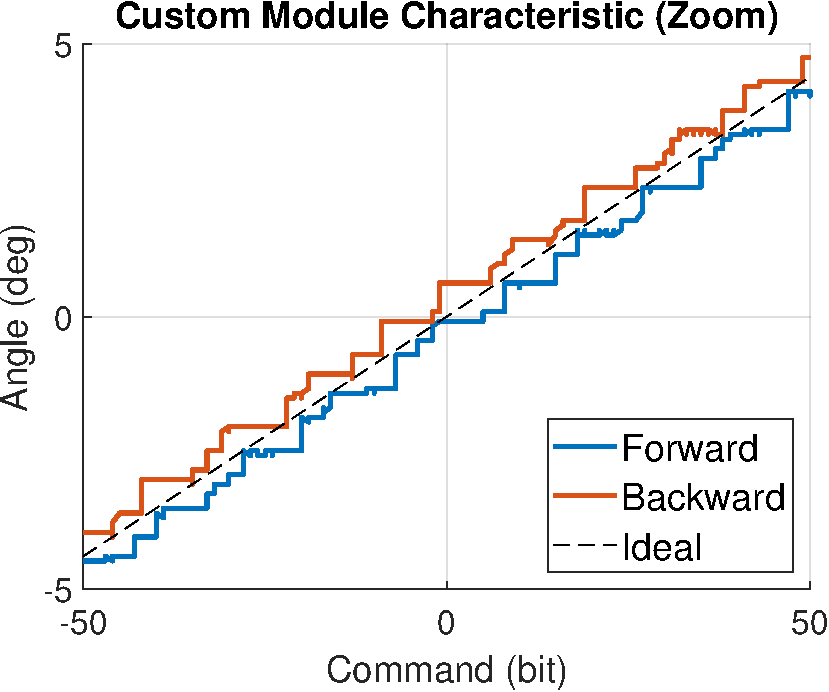
\includegraphics[width=\textwidth]{custom_linearity_zoom.pdf}
            \end{column}
            \begin{column}{0.24\textwidth}
                \centering\footnotesize
                Improvements on:\vspace{10pt}

                Linearity\vspace{10pt}

                Operative Range\vspace{10pt}

                Backlash/Hysteresis\vspace{20pt}

                Micro-scale adjustments without limit cycles\vspace{10pt}

                Settling error $e_\theta \le \pm 1^\circ$
            \end{column}
            \begin{column}{0.38\textwidth}
                \centering
                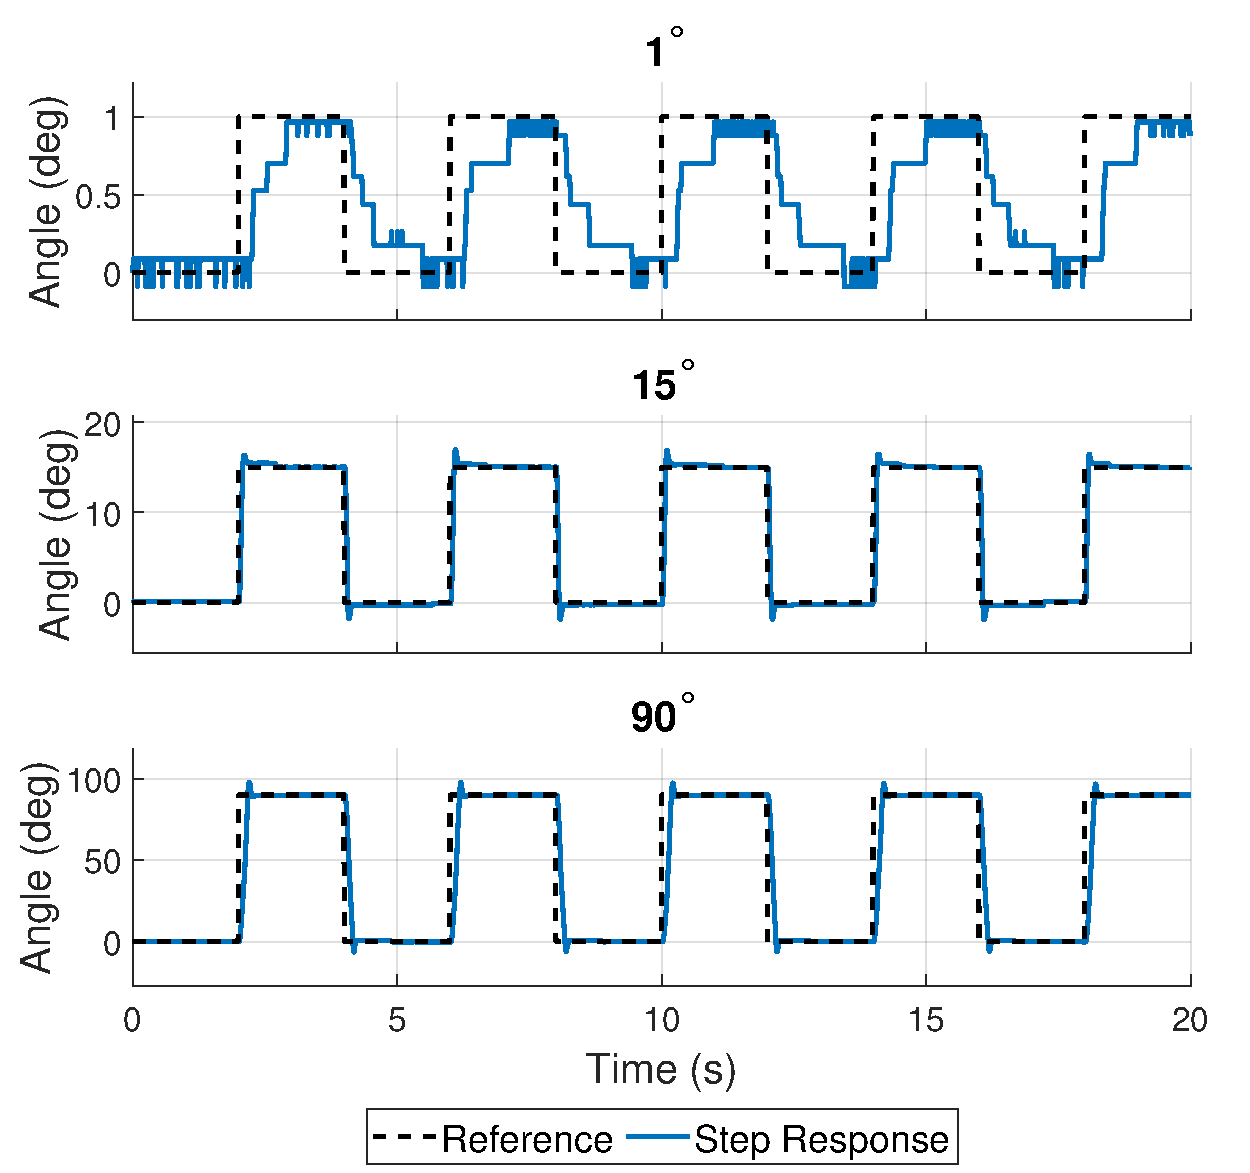
\includegraphics[width=0.9\textwidth]{custom_step_response_multi.pdf}
                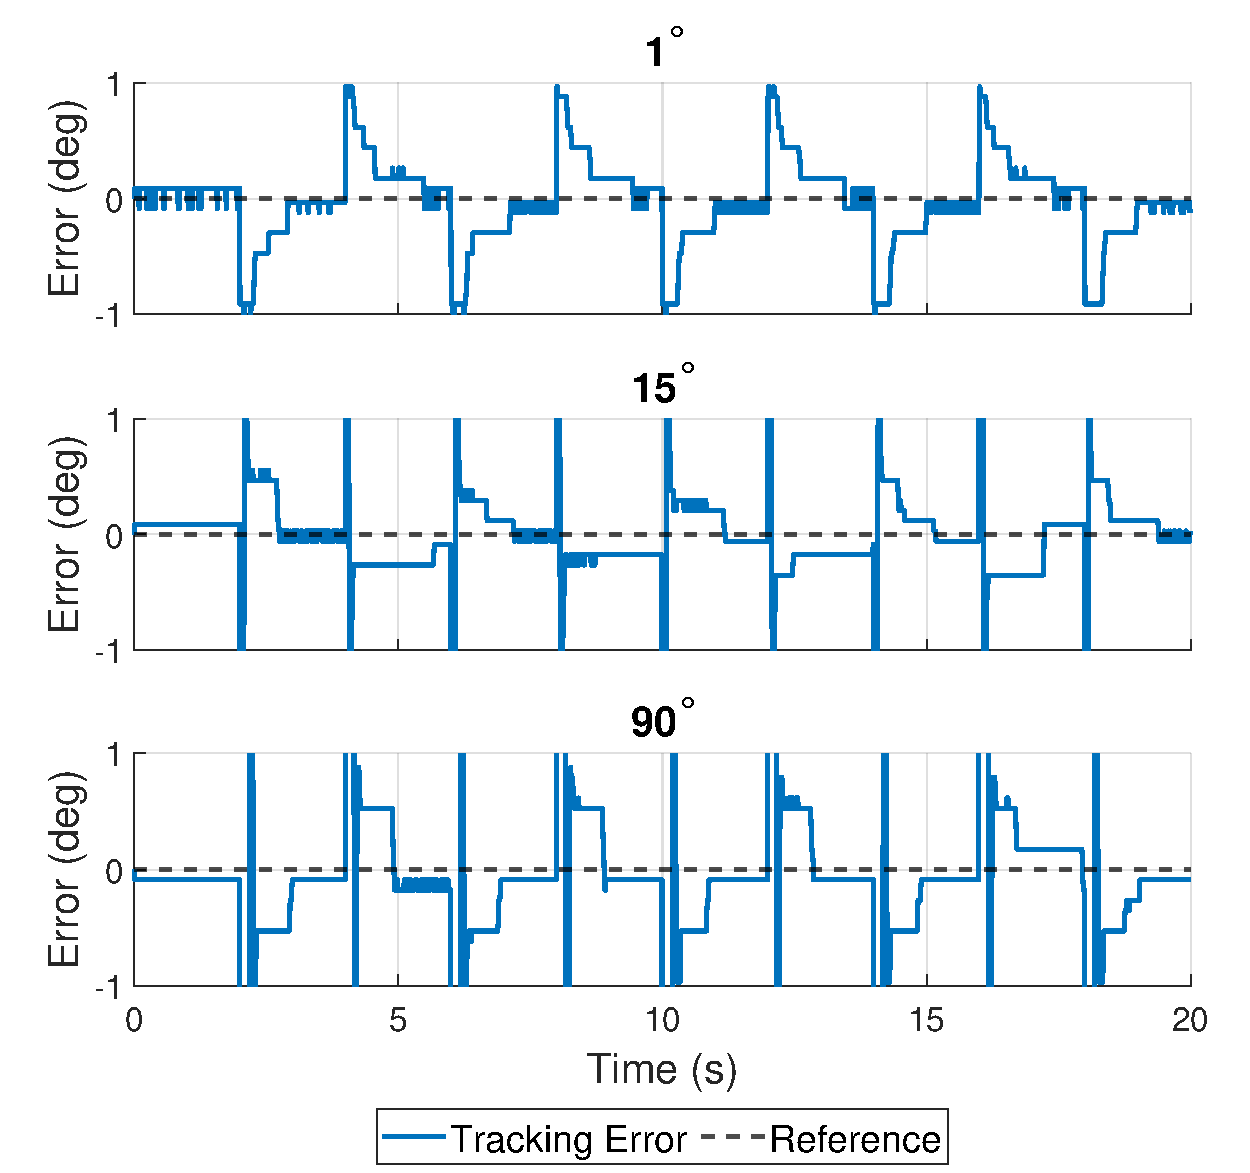
\includegraphics[width=0.9\textwidth]{custom_step_error_multi.pdf}
            \end{column}
        \end{columns}
    \end{frame}

    \begin{frame}{Redesign Metrics}
        \centering
        
\includegraphics[width=0.95\textwidth]{final_benchmark.pdf}

        Price per unit $\le$ 8€ (including components, PCB and shipping)
    \end{frame}

\section{Robotic Limb}

    \begin{frame}{Robotic Limb Design}
        \begin{columns}[c]
            \begin{column}{0.5\textwidth}
                \centering
                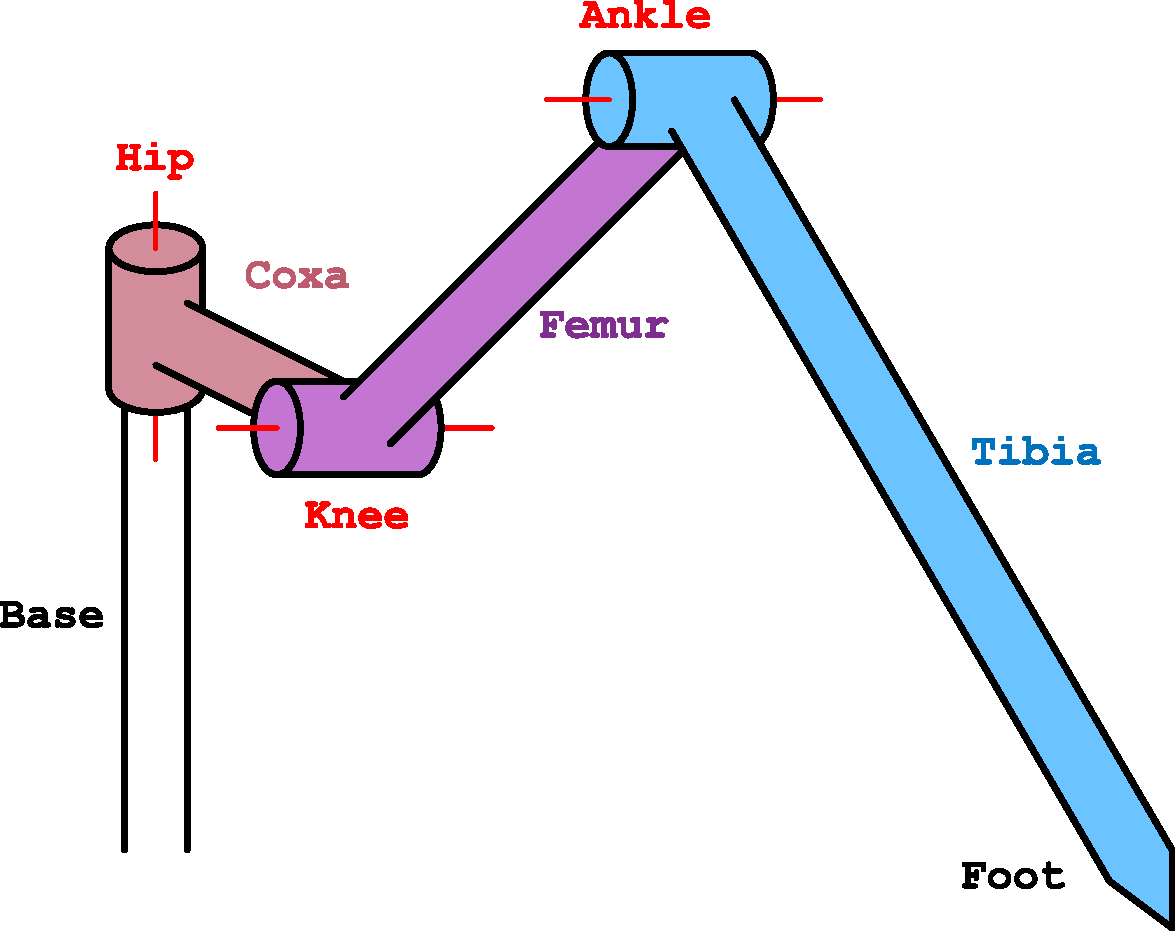
\includegraphics[width=\textwidth]{hexapod-leg.pdf}

                Forward Kinematics\vspace{10pt}

                Inverse Kinematics\vspace{10pt}

                Reachable Workspace
            \end{column}

            \begin{column}{0.50\textwidth}
                \centering
                \reflectbox{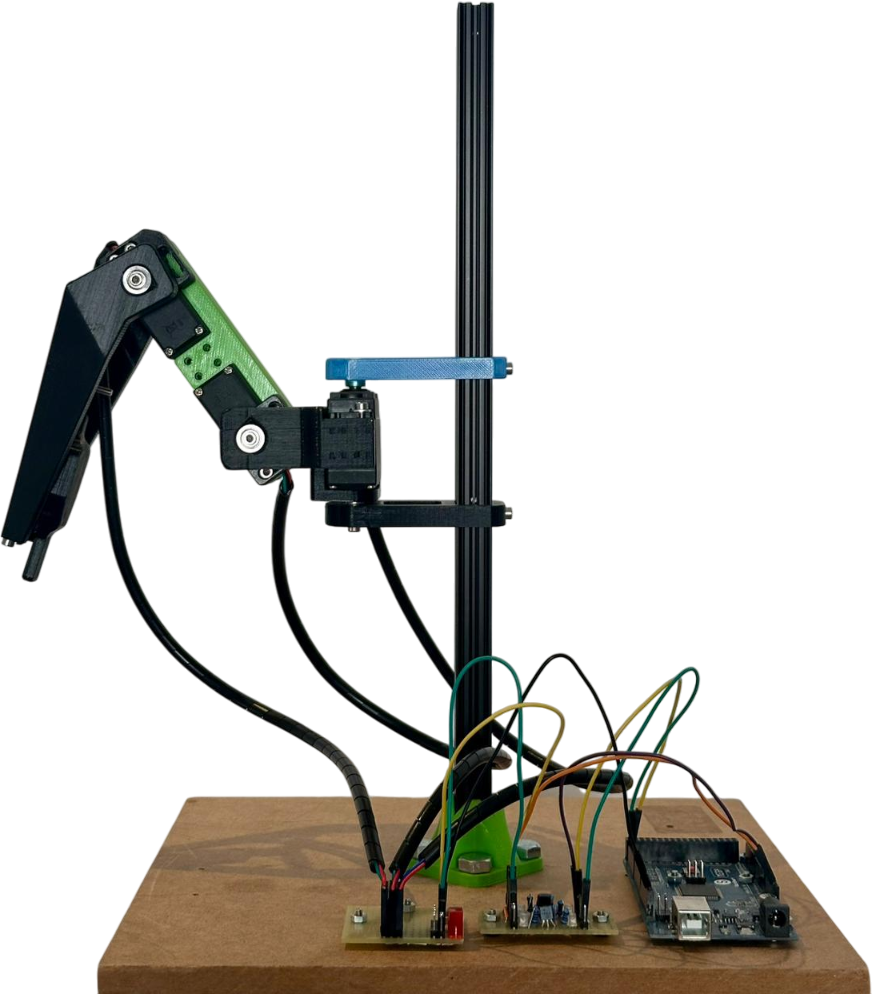
\includegraphics[width=\textwidth]{limb_assembly.png}}
            \end{column}
        \end{columns}
    \end{frame}

    \begin{frame}{Path Generation}
        \begin{columns}[c]
            \begin{column}{0.50\textwidth}
                Assuming \textbf{Flat Ground}\vspace{10pt}

                Geometric derivation parametrized w.r.t. walking speed and direction\vspace{10pt}

                \textbf{Stance Phase:}\\
                Propulsion and constant speed\vspace{10pt}

                \textbf{Swing Phase:}\\
                Repositioning of the foot with no jumps in accelerations
            \end{column}

            \begin{column}{0.5\textwidth}
                \centering
                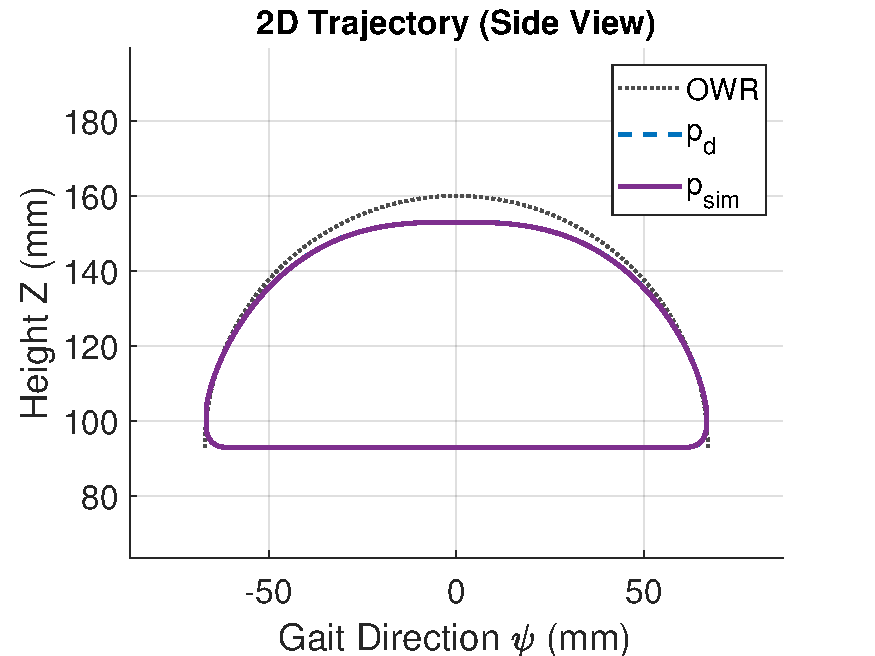
\includegraphics[width=\textwidth]{gait_z_psi.pdf}
            \end{column}
        \end{columns}
    \end{frame}

    \begin{frame}{Simulation and HIL}
        \centering
        Hardware in the Loop Control Chain\vspace{10pt}

        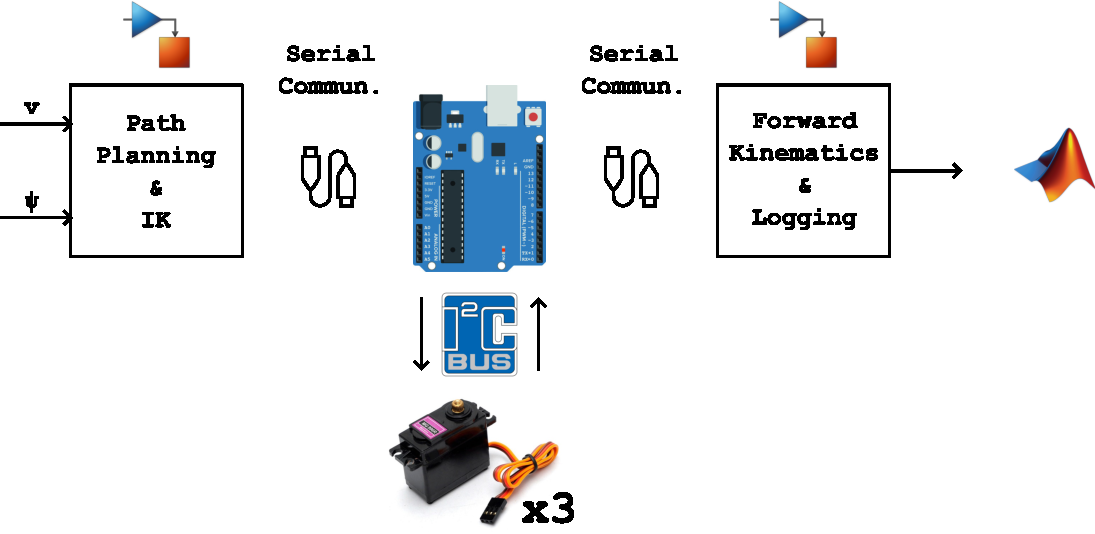
\includegraphics[width=0.70\textwidth]{hil.pdf}

        Simulation Control Chain\vspace{10pt}

        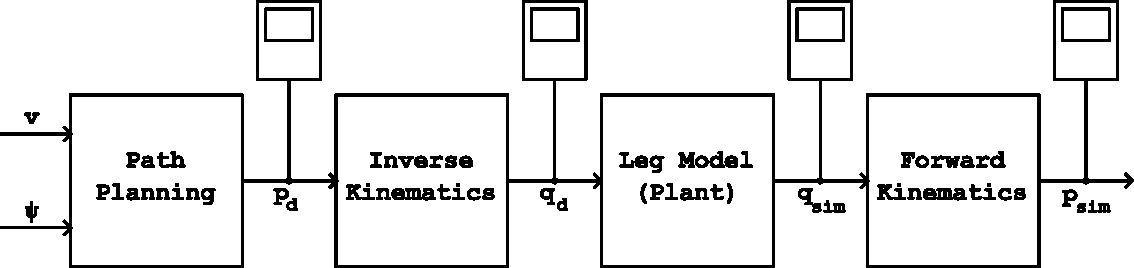
\includegraphics[width=0.70\textwidth]{open_loop.pdf}
    \end{frame}

    \begin{frame}{Robotic Limb Design}
        \begin{columns}[c]
            \begin{column}{0.5\textwidth}
                \centering
                \footnotesize
                Simulation model $\approx$ Physical model\vspace{20pt}

                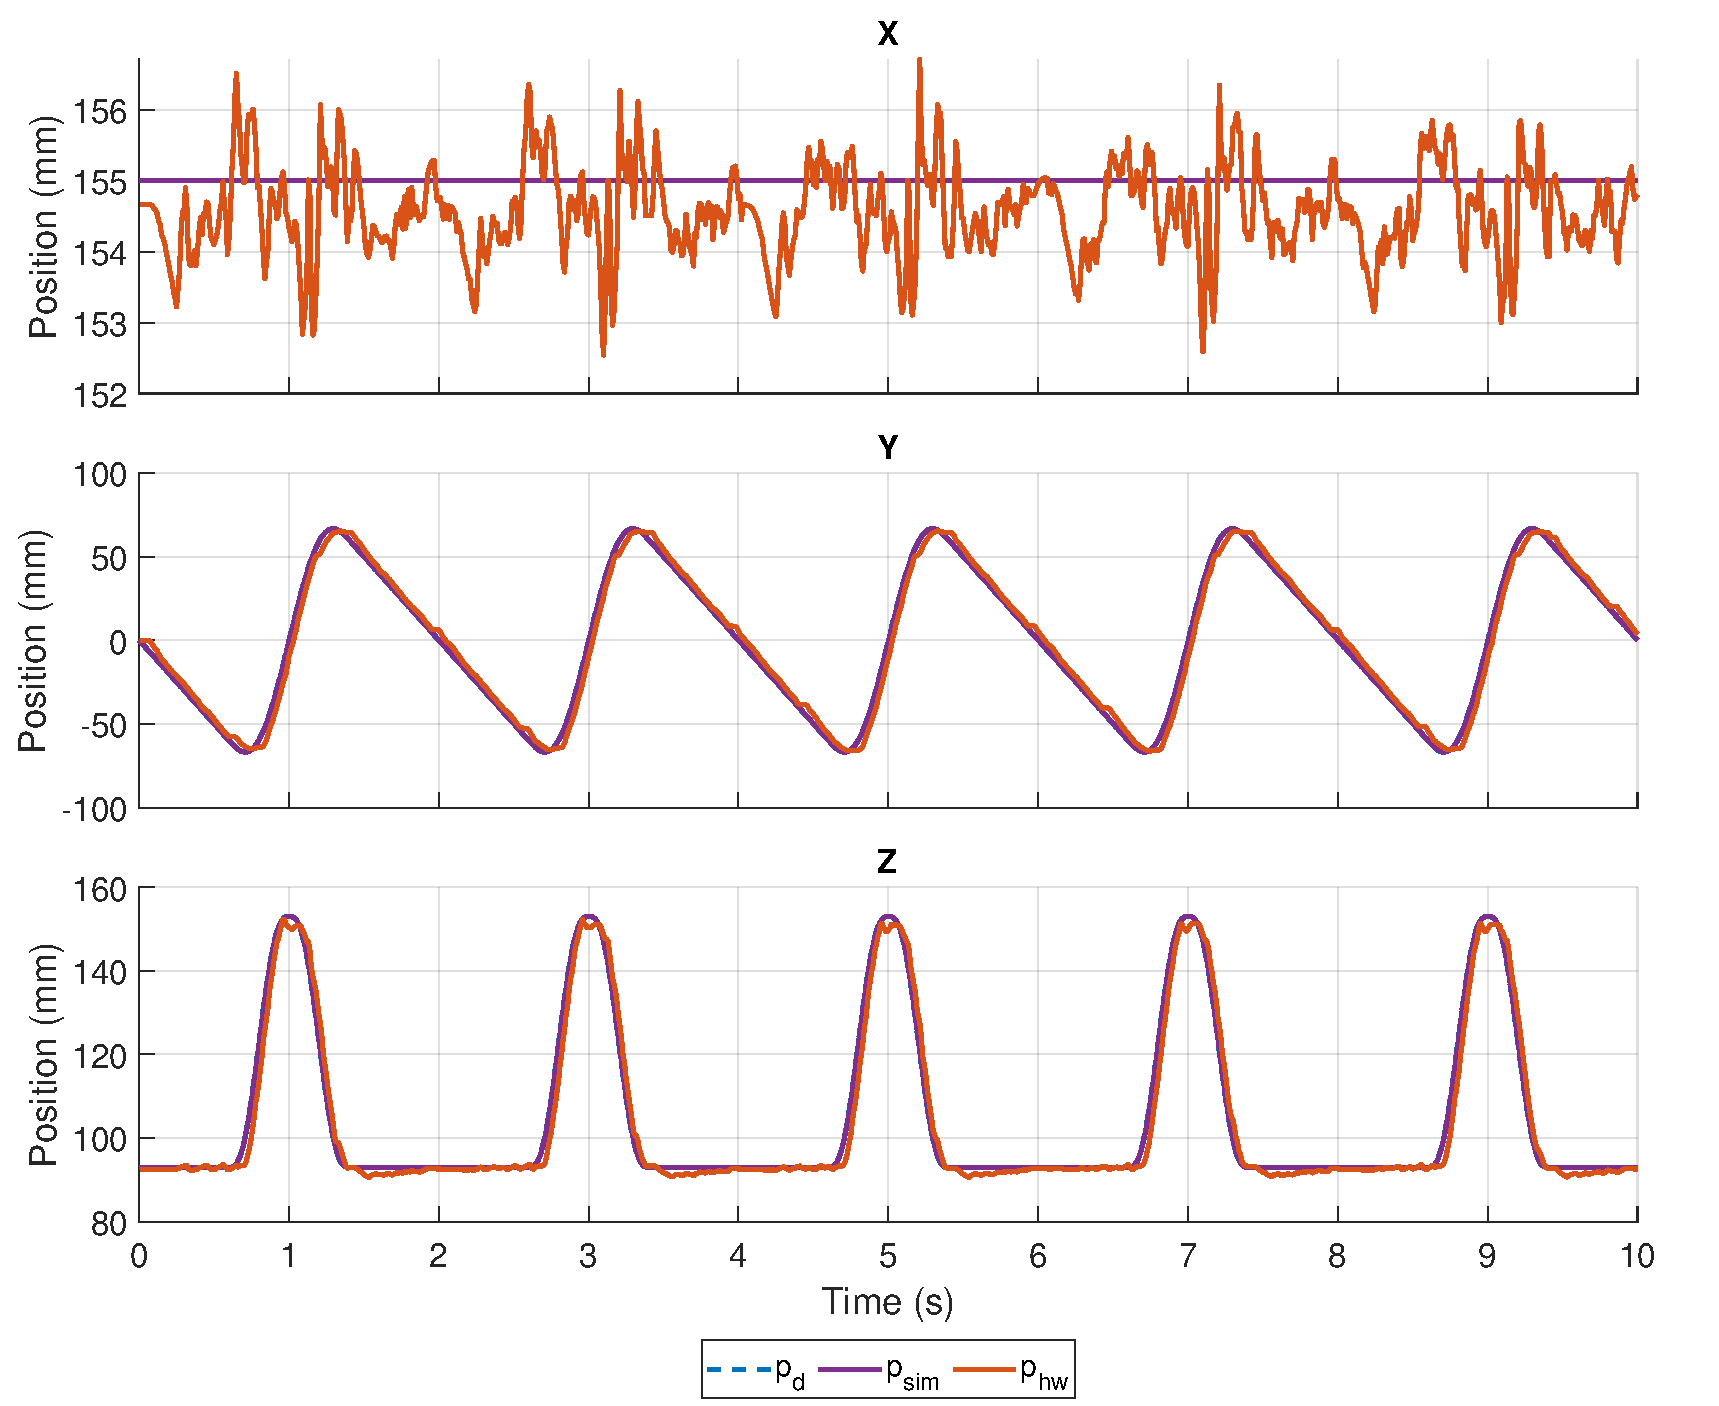
\includegraphics[width=\textwidth]{cartesian_trajectories.pdf}
            \end{column}

            \begin{column}{0.50\textwidth}
                \centering
                % Sintassi: \animategraphics[opzioni]{fps}{percorso/prefisso_nome}{inizio}{fine}
                % loop: ripete all'infinito
                % autoplay: parte appena apri la slide
                % width: larghezza

                \animategraphics[loop, autoplay, width=0.9\textwidth]{20}{experiment/ezgif-frame-}{002}{045}
                % Spiegazione parametri:
                % {10} = Frame al secondo (velocità)
                % {animazione/bot_} = Cerca file tipo "animazione/bot_0.png", "bot_1.png"...
                % {001}{101} = Dal frame numero 1 al numero 101
                (2x)
            \end{column}
        \end{columns}
    \end{frame}

    \begin{frame}{Error Metrics}
        \begin{columns}[c]
            \begin{column}{0.4\textwidth}
            \centering
            Change in \textbf{amplitude} but similar \textbf{shape}, suggesting higher \textbf{tracking delay} in the experiment and \textbf{inertia} effects in both.\vspace{10pt}\\

            Notice the scaling of the simulation error\\(factor of 10)
            \end{column}

            \begin{column}{0.6\textwidth}
            \centering
                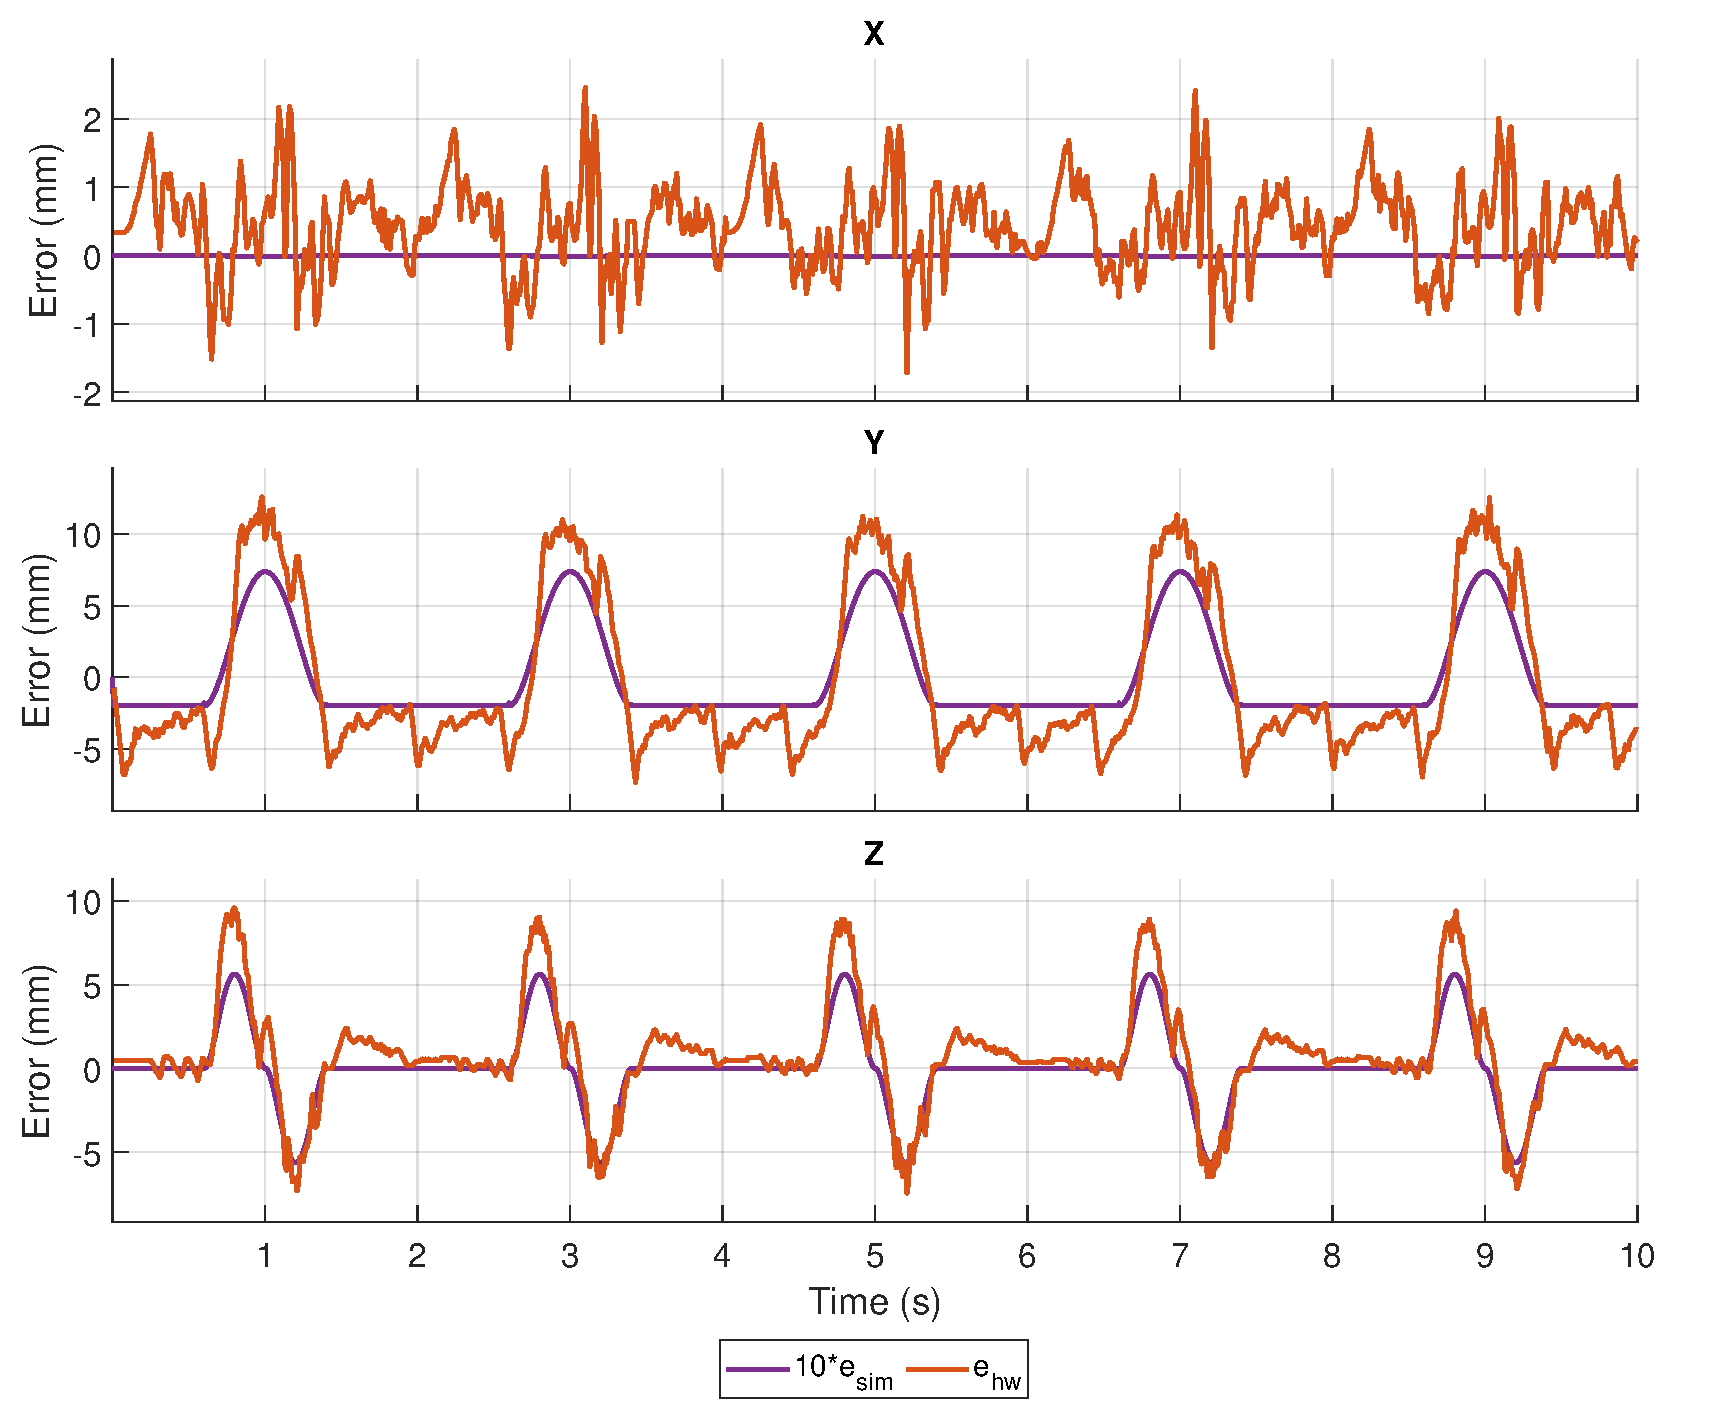
\includegraphics[width=0.8\textwidth]{cartesian_errors.pdf}
                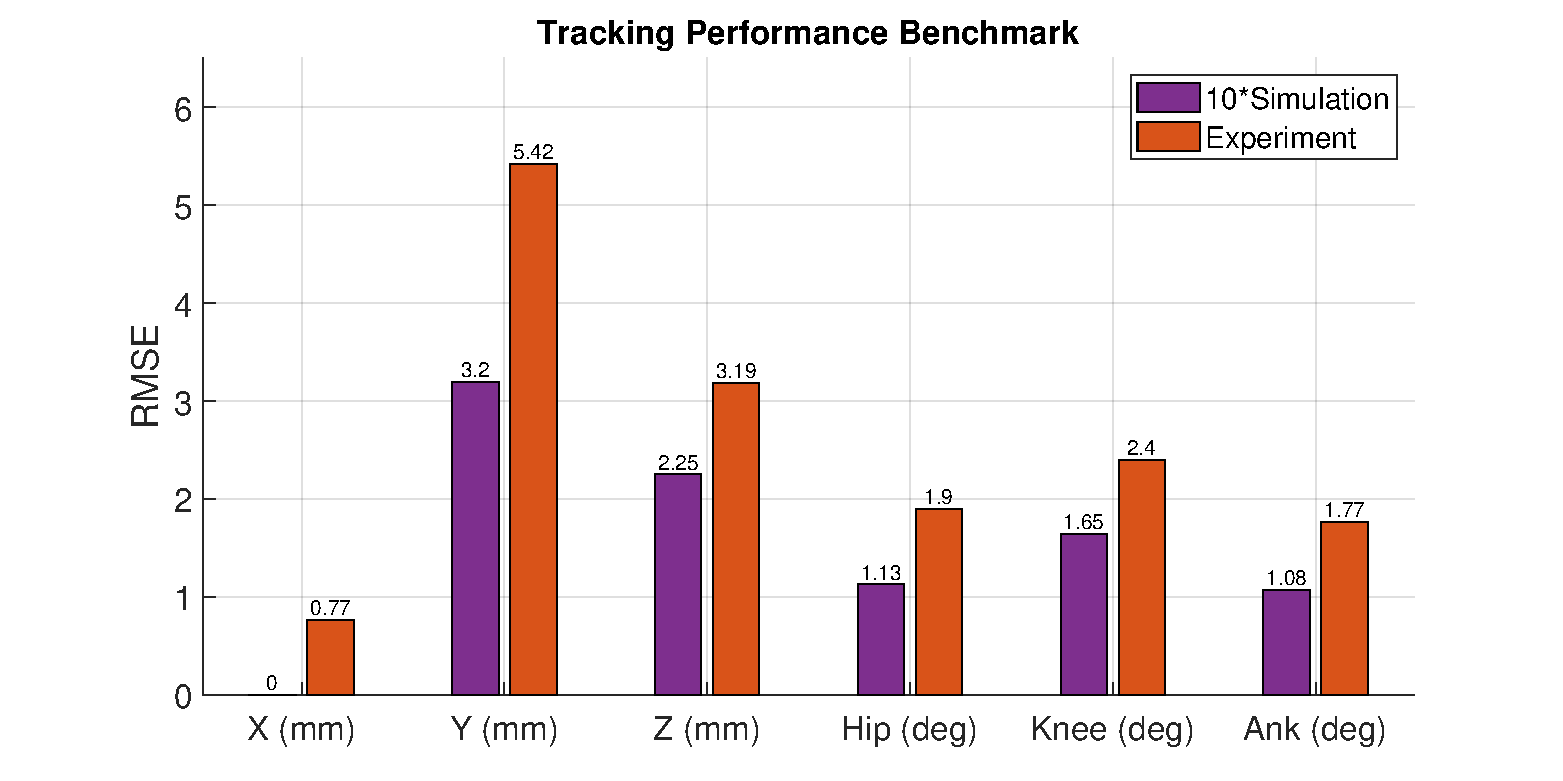
\includegraphics[width=0.85\textwidth]{rmse_benchmark.pdf}
            \end{column}
        \end{columns}
    \end{frame}

    \begin{frame}{Path Adaptation 1/2}
        \begin{columns}[c]
            \begin{column}{0.4\textwidth}
            \centering
            Relaxing the flat ground assumption\vspace{20pt}

            Contact sensor in the Foot\\+\\Adaptive FSM\\Path Generator\vspace{20pt}
            \end{column}

            \begin{column}{0.6\textwidth}
            \centering
                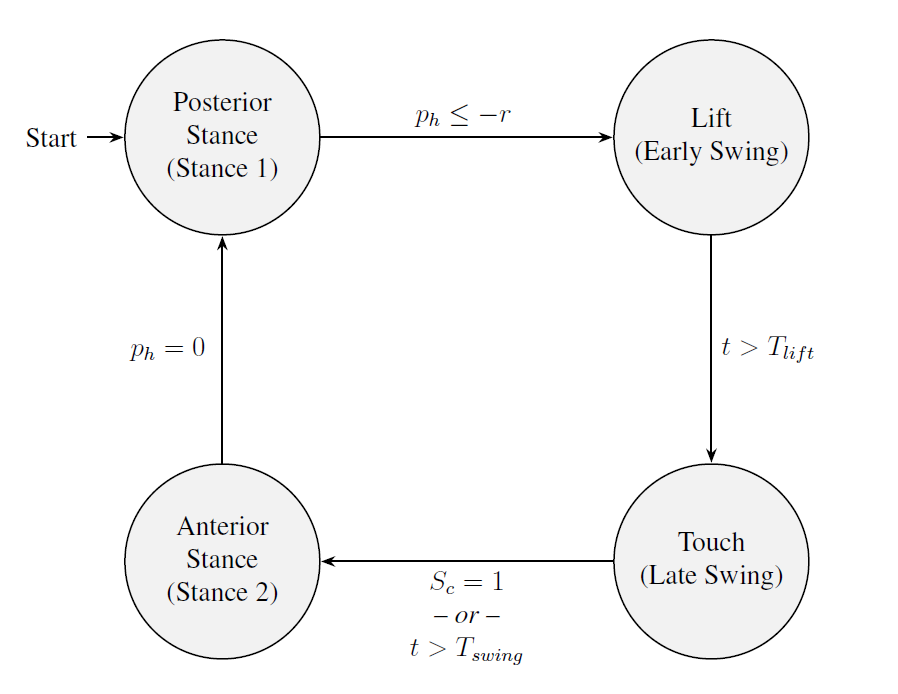
\includegraphics[width=0.8\textwidth]{fsm.PNG}
            \end{column}
        \end{columns}
    \end{frame}

    \begin{frame}{Path Adaptation 2/2}
        \begin{columns}[c]
            \begin{column}{0.5\textwidth}
                \centering
                \footnotesize
                
\includegraphics[width=\textwidth]{adaptive_comparison.pdf}
            \end{column}

            \begin{column}{0.50\textwidth}
                \centering
                % Sintassi: \animategraphics[opzioni]{fps}{percorso/prefisso_nome}{inizio}{fine}
                % loop: ripete all'infinito
                % autoplay: parte appena apri la slide
                % width: larghezza

                \animategraphics[loop, autoplay, width=\textwidth]{10}{animation/ezgif-frame-}{001}{101}
                % Spiegazione parametri:
                % {10} = Frame al secondo (velocità)
                % {animazione/bot_} = Cerca file tipo "animazione/bot_0.png", "bot_1.png"...
                % {001}{101} = Dal frame numero 1 al numero 101
            \end{column}
        \end{columns}
    \end{frame}

\section{Conclusions}

    \begin{frame}{Final Considerations}
        Complete design of the 3-DOF robotic limb, from micro-scale components (custom actuator) to macro-scale system (full limb), including the control chain.\vspace{10pt}

        Excellent results with a contained budget, also applicable to similar projects.\vspace{10pt}

        Solid foundations for future improvements:
        \begin{enumerate}
            \item Automatic controller gain tuning;
            \item Full robot  assembly;
            \item Adaptive path generator testing and refinement;
        \end{enumerate}
    \end{frame}

    \begin{emptyframe}
        Thank you!\\Questions?
    \end{emptyframe}

\section*{Extra}

    \begin{frame}{Metrics}
        \centering
        $$\text{RMSE} = \sqrt{ \frac{1}{N} \sum_{i=1}^{N} \left( y_{meas}[i] - y_{ideal}[i] \right)^2 }$$

        $$E_{max} = \max_{i} \left| y_{meas}[i] - y_{ideal}[i] \right|$$

        $$\mathcal{A}_{hyst} = \int_{x_{min}}^{x_{max}} \left| \left( y_{fwd}(x) - y_{bwd}(x) \right) \right|\, dx $$

        $$H_{avg} = \frac{\mathcal{A}_{hyst}}{x_{max} - x_{min}}$$
    \end{frame}

\end{document}